
%%%%%%%%%%%%%%%%%%%%%%%%%%%%%%%%%%%%%%%%%%%%%%%%%%%%%%%%%%%%%%%%%%%%%%%%%
%           Capítulo 2: MARCO TEÓRICO - REVISIÓN DE LITERATURA
%%%%%%%%%%%%%%%%%%%%%%%%%%%%%%%%%%%%%%%%%%%%%%%%%%%%%%%%%%%%%%%%%%%%%%%%%
\chapter{Background}

This chapter presents the main background of the wing-integrated aircraft. Its first designs, features, advantages and main challenges. Finally, a brief description of the flight control systems of the main Boeing and Airbus scale models is given. 


%%%%%%%%%%%%%%%%%%%%%%%%%%%%%%%%%%%%%%%%%%%%%%%%%%%%%%%%%%%%%%%%%%%
\section{Blended-Wing-Body Aircraft}

Aviation is a global point of interest, where one of the aspects that have taken the attention of major aerospace companies such as Boeing and Airbus is its environmental impact. Among the main sources of pollution we have noise, carbon dioxide polluting emissions ($CO_2$) and nitrogen oxides ($NOx$). 
%
In the Figure \ref{fig: emisiones de la aviación comercial} we can observe the contrast of the emissions of $CO2$ global compared to those emitted by commercial aviation on a timeline until 2015. Emissions from commercial aviation contribute to the  $2\%$ of global emissions.
%
\begin{figure}[h]
\centering
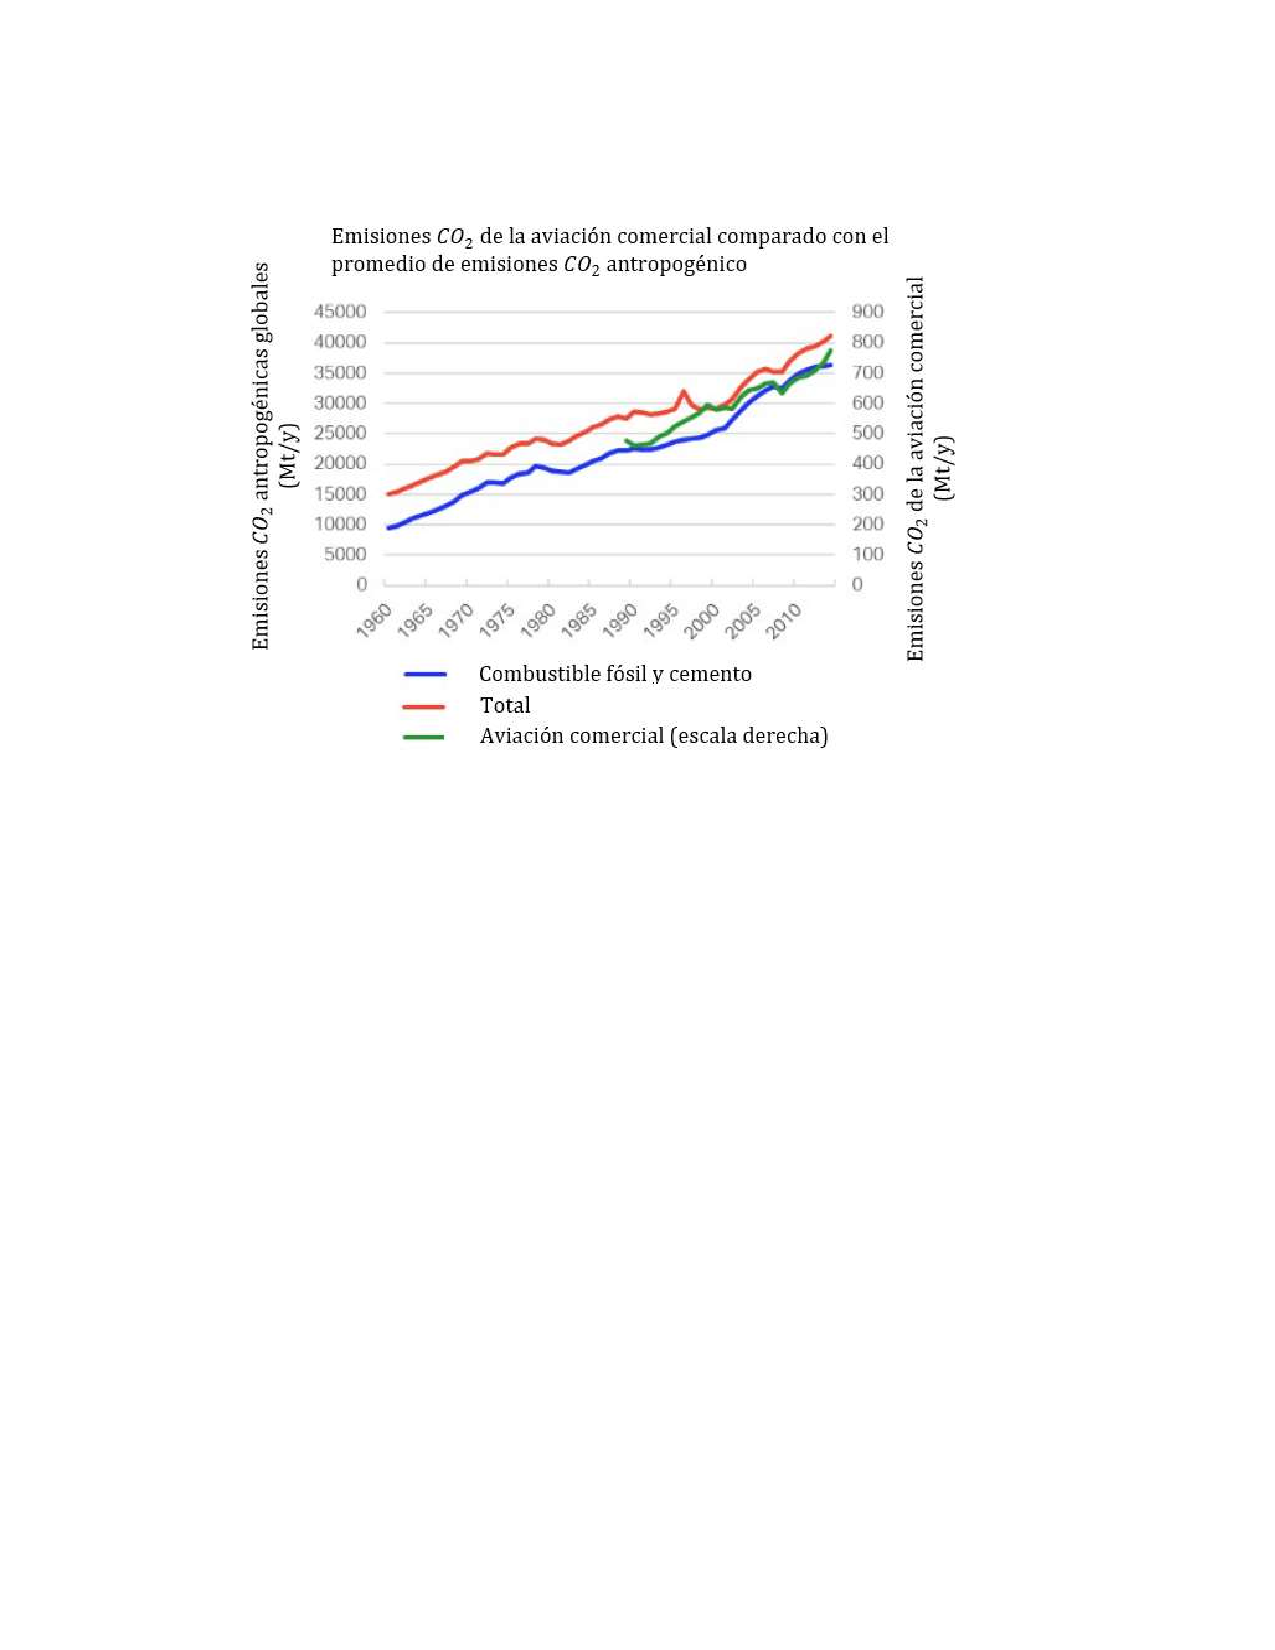
\includegraphics[scale=0.75]{Capitulo3/figs/emsisiones CO2 global y aviacion_cropped.pdf}
\caption{Emisiones $CO_2$ Global anthropogenic and commercial aviation  \cite{IATA2020}}
\label{fig: emisiones de la aviación comercial}
\end{figure}
%
Also, based on the annual reports of Boeing and Airbus \cite{OneAir}, it is observed that in the last 15 years the number of passengers using an aircraft has tripled. 
%
In 2019 alone, 4.5 million people traveled on one of the 1300 airlines that total 26,000 aircraft around the world, and which made 40 million flights in that year alone.
%
In addition, according to a study by Airbus and the International Civil Aviation Organization (\textit{ICAO}) a forecast of how between 2021 and 2041 will vary the passengers-kilometer (\textit{RPK, in English}), ver Figura \ref{pronostico RPK 2021-2041}.
%
\begin{figure}[h]
\centering
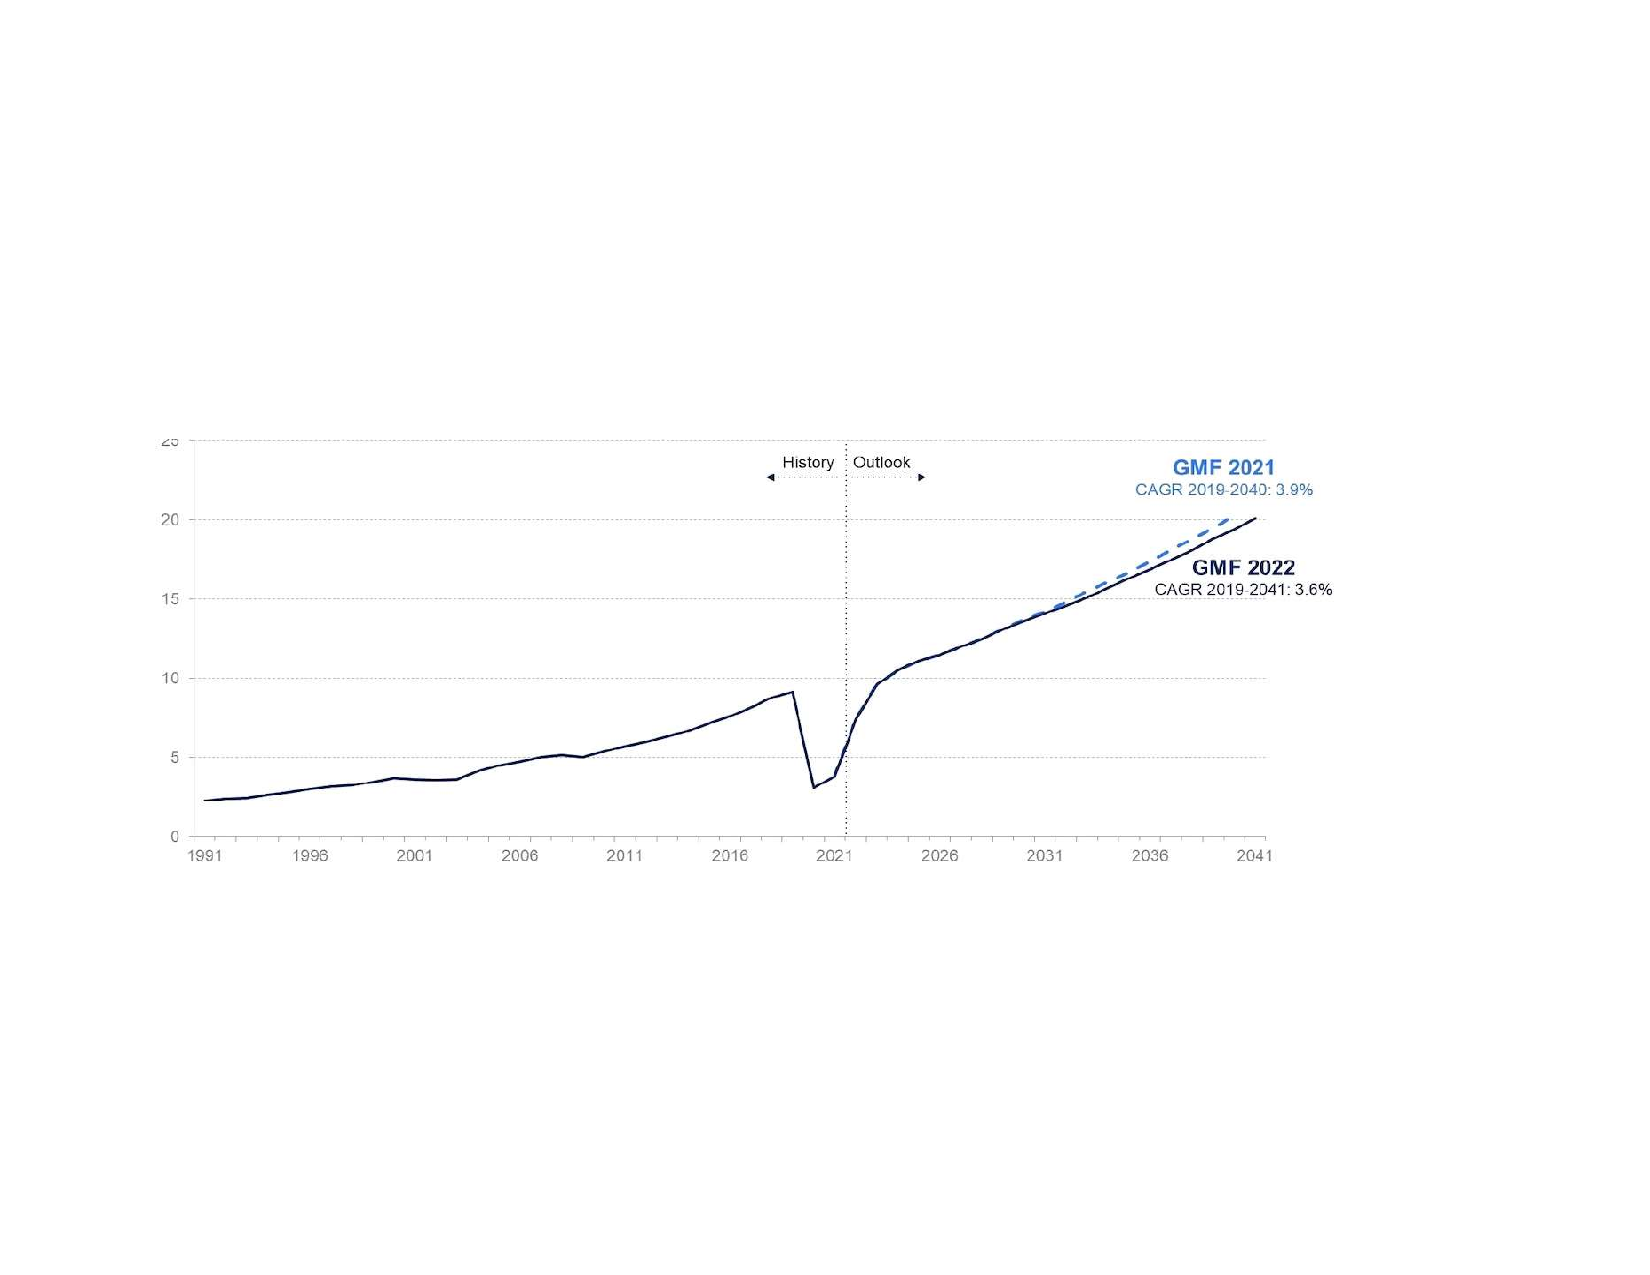
\includegraphics[scale=0.6]{Capitulo3/figs/pronostico AirbusICAO 2041_cropped.pdf}
\caption{Forecast in trillions of revenue per passenger-kilometre 2021-2041\cite{OneAir}}
\label{pronostico RPK 2021-2041}
\end{figure}
%

As actions to address this problem, since 2009 the entire aviation industry (airlines, aerospace manufacturing companies, airports, navigation service providers and aviation business) has set high-level climate targets:
\begin{itemize}
    \item Improving fuel efficiency in $1.5 \%$ per year between 2009-2020. 
    \item Achieve net neutral carbon emissions growth from 2020 onwards.
    \item Reduce net global carbon emissions by $50 \%$ per cent by 2050 compared to 2005. 
\end{itemize}
%
%
It is important to mention that reducing pollutant emissions is a challenge that requires a combination of all possible contributions from stakeholders and on all pillars of the International Air Transport Association (IATA) strategy. 
%
In this sense, it is considered that from 2035 onwards, radical and innovative technologies with high efficiency in performance and fuel could be realized such as new aircraft configurations on the current conventional TAW, and new forms of energy sources for the propulsion system; such as electric batteries, hydrogen cells and hybrid proposals. 
%
In the Figure \ref{tecnologías evolutivas y revolucionarias} the possible technological advances in aviation categorized as evolutionary and revolutionary in the period 2020-2050 are shown.

Within the current context of aircraft we have the main \textbf{evolutionary technological developments in the air} will be implemented in a conventional TAW configuration with jet turbofan fossil fuel engines. The list of the main technological evolutionary contributions is in the groups of new architectures in engines and new advanced concepts, in engine cycles, in aerodynamics and in different systems. From the above, it is considered that new engine technologies can improve between a $10\%$ and a $25\%$ fuel efficiency, \cite{IATA2020}.

On the other hand, we have the group of \textbf{revolutionary technological aerial advances} Within this group, aircraft with new configurations in geometry are considered to be the main differentiator, such as wing-integrated aircraft, combined with material innovation and the morphology of their structures. It is also considered a revolution in propulsion with open rotors as well as the implementation of limit layer actuators as agents of high improvement. 
%
The most prominent and expected impact is on clean power sources for propulsion and aircraft systems, where hybrid, electric and hydrogen proposals see low or emission-free aviation. In this thesis work we are interested in the design and control of an integrated aircraft, BWB.
%
\begin{figure}[h]
\centering
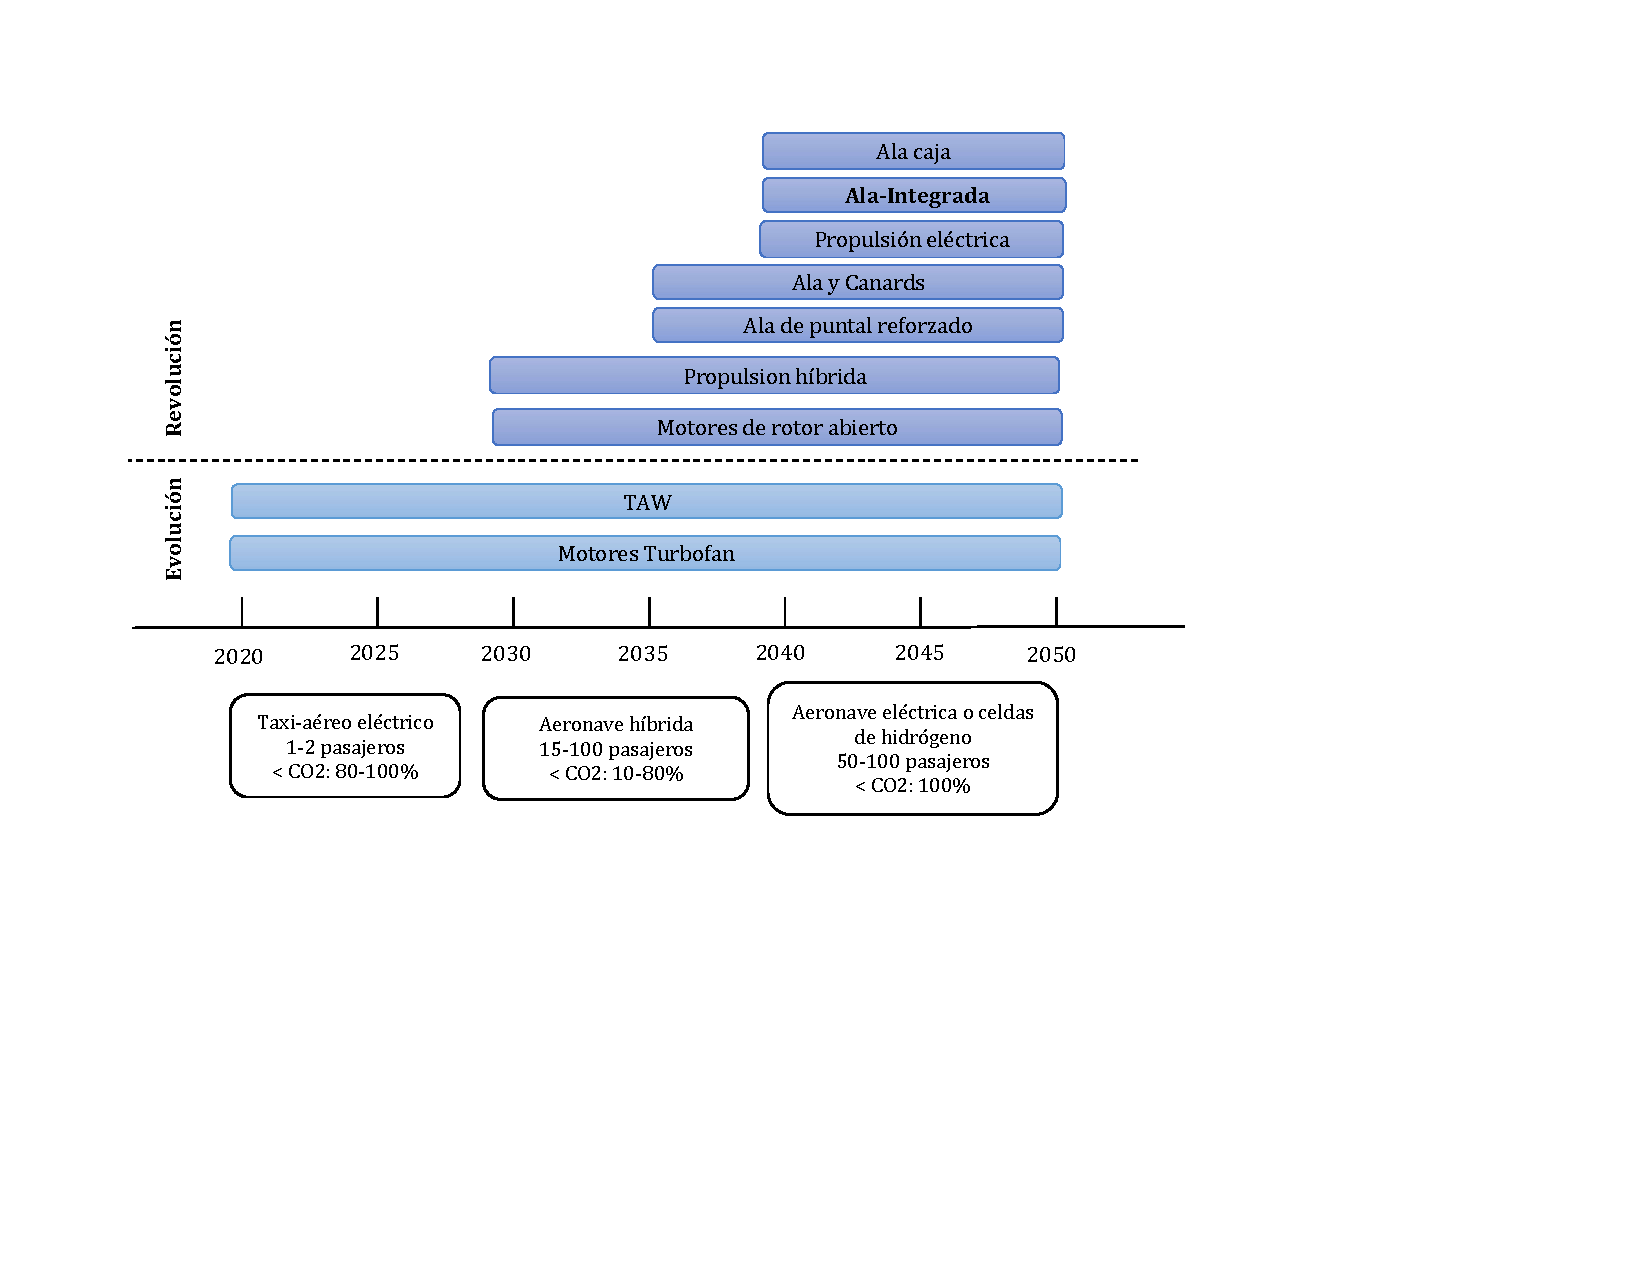
\includegraphics[scale=0.63]{Capitulo3/figs/Aviacion evolucion revolucion_cropped.pdf}
\caption{2020-2050 forecast of evolutionary and revolutionary technologies in aviation \cite{IATA2020}}
\label{tecnologías evolutivas y revolucionarias}
\end{figure}
%

%%%%%%%%%%%%%%%%%%%%%%%%%%%%%%%%%%%%%%%%%%%%%%%%%%%%%%%%%%%%%%%%%%%%%%
%
Timothy Risch, leader of the NASA X-48 BWB project, considers that the wing-integrated aircraft is an aircraft configuration characterized by an overall design with minimal distinctions between wing and fuselage. A wing-integrated aircraft looks like a wing-integrated aircraft but concentrates a larger volume in Delta form in its central section, long enough for a passenger cabin, which is integrated into the wing panels, see Figure \ref{fig: configuraciones de aeronaves}. The forecast for BWB improvement compared to TAW in fuel performance is estimated above the $27\%$. 
%
\begin{figure}[h]
\centering
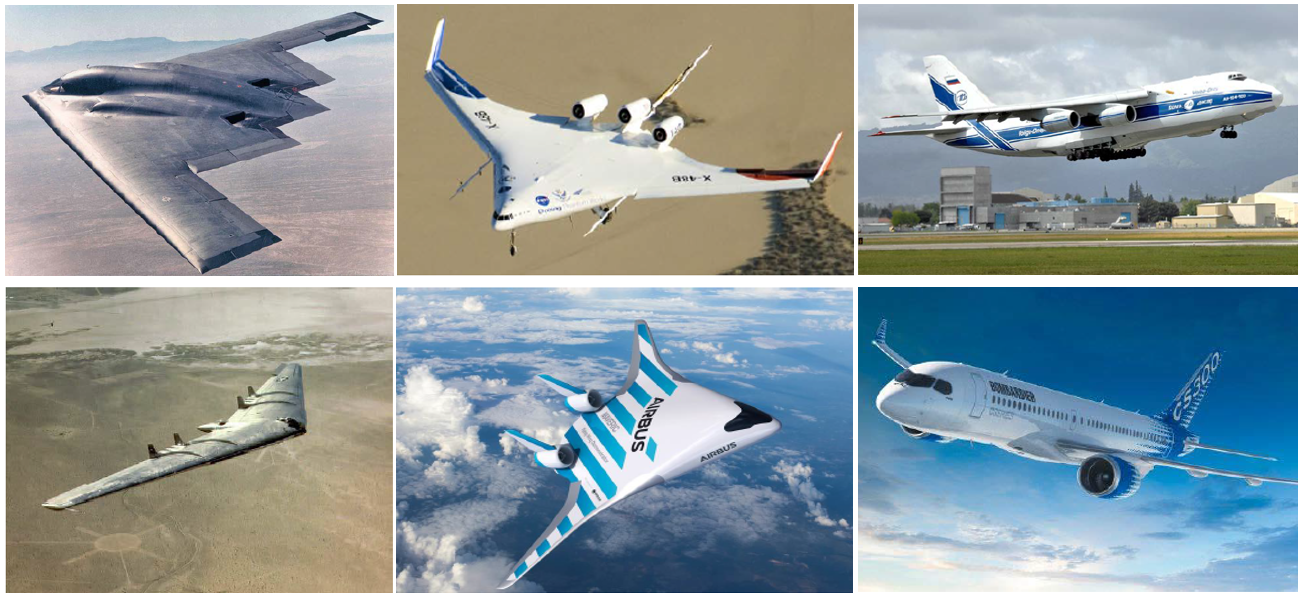
\includegraphics[scale=0.5]{Capitulo3/figs/2 5.png}
\caption{Aircraft configurations: Wing-Flying (FW), Wing-Integrated (BWB) and Tube-Wing (TAW)}
\label{fig: configuraciones de aeronaves}
\end{figure}
%

In \cite{IATA2020}, according to a methodology of the German Aerospace Center (DLR) is estimated the potential savings in carbon emissions $CO_2$ according to different scenarios of technological implementation:
\begin{enumerate}
    \item $T1$: Imminent technologies. Obvious improvements in current technology close to launch.
    \item $T2$: Conservation technologies. Improvements in turbofan engines without radical changes.
    \item $T3$: Radical technologies. New turbofan engines and open rotors. Substantial improvements to new configurations (e.g. BWB).
    \item $T4$: Technologies beyond. Additional improvements to new configurations (T3), low-emission hybrid systems, and emission-free electric and hydrogen systems, energy $100\%$ renovables. 
\end{enumerate}
%DLR propone 8 categorías de asientos para pasajeros: 1) 51-100, 2) 101-150, 3) 151-210, 4) 211-300, 5) 301-400, 6) 401-500, 7) 501-600, 8) 601-650. 
%
All scenarios range from a fuel saving of $27\%$ up to and including $100\%$. Improvements $T1,T2$ in TAW and its turbofan engines are listed with an impact between $27-45 \%$while the BWB aircraft is on the scene $T3,T4$ with significant improvements in fuel saving, having the ability to achieve a $100\%$ in its electrical and hydrogen cell versions.
%
\begin{figure}[h]
\centering
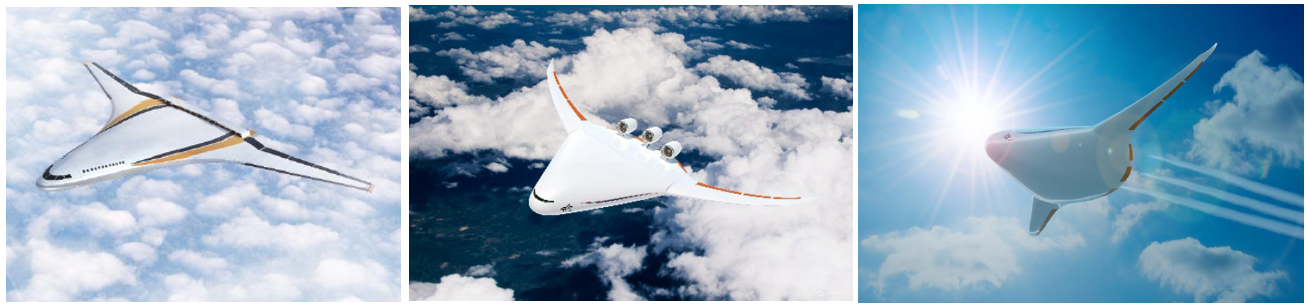
\includegraphics[scale=0.5]{Capitulo3/figs/2 3.png}
\caption{NASA-BWB turbo-electric and DLR-BWB  \cite{IATA2020}}
\label{fig: NASA-BWB y DLR-BWB}
\end{figure}
%
%
However, the design of a BWB aircraft requires a high integration of preliminary analysis.
%%%%%%%%%%%%%%%%%%%%%%%%%%%%%%%%%%%%%%%%%%%%%%%%%%%%%%%%%%%%%%%%%%%%%%%
% Estrategias de diseño en propulsión y estructura

In \cite{Kumar2017} the design and analysis of the location and number of engines for a BWB aircraft is presented. As a result of this design it is obtained that the location of the engines above the body BWB improves the lifting/drag ratio in a $10 \%$. In addition, the base of a wing-integrated aircraft is ideal for having a propulsion system of intake of the boundary layer (BLI) and/or distributed propulsion systems. This allows it to be maneuverable at the cost of over-acting control.
%
\begin{figure}[!h]
\centering
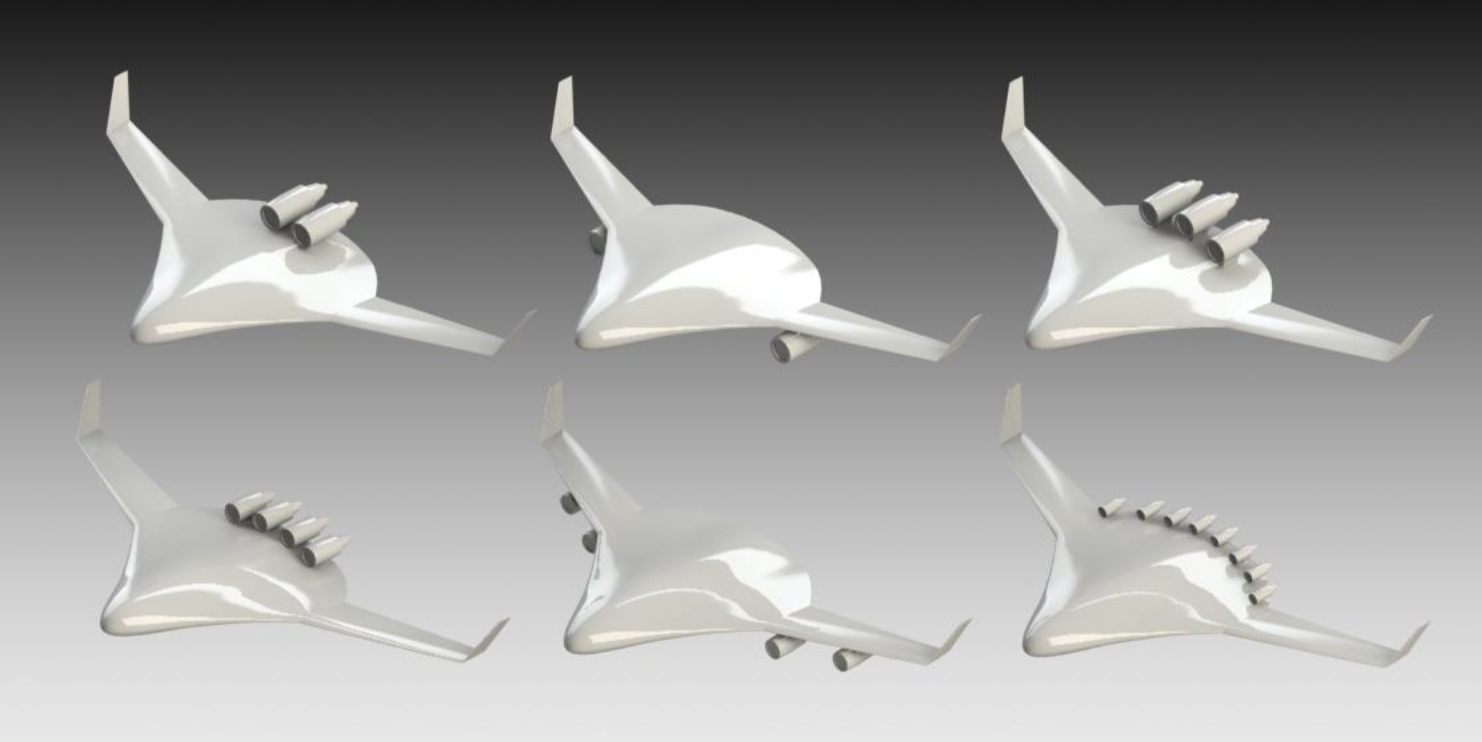
\includegraphics[scale=0.35]{Capitulo3/figs/2 4.png}
\caption{Wing-Integrated and distributed propulsion options  \cite{Kumar2017}}
\label{fig: propulsion distribuida}
\end{figure}
%
The distributed propulsion implementation allows the implementation of vector thrust control systems by replacing aerodynamic control surfaces, since both devices are located at the trailing edge. 
%
Additionally, as part of this work we analyzed six propulsion options for BWB: 1) two engines above, 2) two engines below, 3) three engines above, 4) four engines above, 5) four engines below and 6) eight engines above, see Figure \ref{fig: propulsion distribuida}Although it was concluded that there is no optimal propulsion system for BWB; it is mentioned that the eight engine model is the best aerodynamic performance, the three engine model is ideal for maximum take-off weight, the two engine model is the optimal case for empty weight, and the four engine model is the most efficient in specific thrust fuel consumption. 
%
In contrast, the configurations of three and four engines have a long disruption of the air flow, generating turbulence and an increase in the drag. More engines still of considerable size (3-4 engines) decrease the aerodynamic performance.
%
On the other hand, it is argued that both two and eight engines are the promise of the future for BWB, but at the same time, the author bets even more on the propulsion of eight engines given their best results in ratio lift/drag, aerodynamic performance and lower maximum take-off weight; in contrast to the worst choice in specific fuel consumption. 
%
Since the analysis used existing engines, it is argued that engines designed for a particular BWB aircraft, with new materials and technology can make the configuration of eight engines the most efficient in this configuration. However, pending that technology the location of two engines would be the most viable option with the best performance. 


In \cite{Panagiotiu2017}, the aerodynamic design of unmanned BWB aircraft is studied to select the optimal structural combination where the main objective is to achieve both performance as well as aerodynamic stability and control.
%
\begin{figure}[!h]
\centering
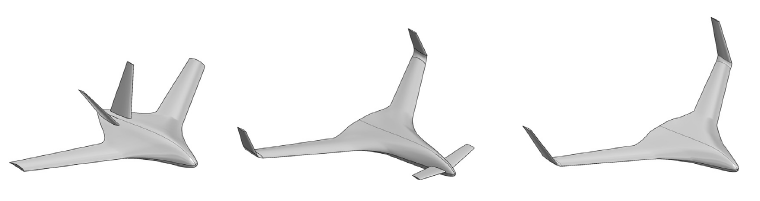
\includegraphics[scale=0.8]{Capitulo3/figs/2 9.png}
\caption{BWB configurations for aerodynamics and control: 1) Vertical stabilizer in V, 2) Canards and 3) Tip fins \cite{Panagiotiu2017}}
\label{fig: configuraciones BWB aero y control}
\end{figure}
%
Three configurations are proposed for stability and control: 1) vertical stabilisers in V for stability and longitudinal and directional control, 2) canards for stability and longitudinal control and 3) fins on tips for stability and directional control, see Figure \ref{fig: configuraciones BWB aero y control}. 
%
The three configurations have elevons on the trailing edge to generate the pitching and rolling moments. While the three configurations provide good metrics given a low drag and a high lift/drag ratio, model 3) presents the best lift coefficient. Configuration 1) would be the least efficient model in aerodynamics, given the drag generated by the V stabilizers. 
%
In terms of stability, given the great capacity we have in the internal volume, it is possible to locate the center of gravity where it best suits. Aerodynamic profiles should also be selected that allow to adapt the internal volume of payload and aircraft systems such as tanks, cells or energy batteries.
%
Aerodynamic profiles with comba are used for longitudinal stability purposes, seeking to reduce the moment of pitching downwards, which if not met, would increase the requirements for the \textit{trimming} o Balancing flight, which in turn generates greater drag and energy consumption of control inputs. 

\medskip

According to \cite{CHEN2019}, it is possible to mention the following: \textbf{Benefits of BWB}:
\begin{itemize}
    \item Reduction of friction drag by a smaller area of contact with the fluid considering the same volume, the compensation drag can be avoided by adopting a relaxed stability in the pitching, reduction of the interference drag thanks to a harmonious assembly central-wing body, reduction of the drag induced by grace support to an elevation distribution throughout the vehicle, reduction of the wave drag at transonic speed due to a better aerodynamic morphology., simplification in the hyper-sustenting devices, in the reduction of the wing weight and a better margin at high-altitude thanks to the reduction of the wing load, allows the location of the engines above the central body which significantly reduces the noise produced, the relief of the local aerodynamic load by means of the local inertia load can reduce the loads of bending and cutting in the structure, the simplicity of the configuration suggests a reduction in manufacturing costs.In addition, BWB is an ideal configuration for laminar flow technology, adjustable configuration for high-capacity applications and significant cost reduction in direct operations can be achieved.
\end{itemize}
%\begin{itemize}
%    \item Reducción del arrastre de fricción por una menor área de contacto con el fluido considerando un mismo volumen.
%    \item El arrastre de compensación puede evitarse adoptando una estabilidad relajada en el cabeceo.
%    \item Reducción del arrastre de interferencia gracias a una armonioso ensamble cuerpo central-ala.
%    \item Reducción del arrastre inducido por lift gracia a una distribución de levantamiento en todo el vehículo.
%    \item Reducción del arrastre de olas a velocidad transónica debido a una mejor morfología aerodinámica.
%    \item Simplificación en los dispositivos hiper-sustentadores, en la reducción del peso de ala y un mejor margen a alta-altitud gracias a la reducción de la carga alar. 
%    \item Permite la ubicación de los motores encima del cuerpo central lo que reduce significativamente el ruido producido.
%    \item El alivio de la carga aerodinámica local mediante la carga de inercia local puede reducir las cargas de flexión y de corte en la estructura.
%    \item La simplicidad de la configuración sugiere una reducción en los costos de manufactura.
%    \item Configuración ideal para tecnología de flujo laminar.
%    \item Configuración ajustable para aplicaciones de alta capacidad. 
%    \item Reducción significativa de costos en operaciones directas pueden lograrse.
%\end{itemize}
%
Asimismo, algunos \textbf{Challenges of BWB} or open problems are:
\begin{itemize}
    \item It requires a relaxed static stability and a \textbf{Automatic flight control system} to fly efficiently, weight penalty due to a pressurized non-circular cabin, lower flight and maneuver qualities due to relaxed stability, limited control authority and complex flight control system design, recovery capacity for potential falls on unembarked aircraft, fewer windows reflected in less comfort for passengers on commercial flights, meeting evacuation requirements and certificates of navigability, wind gust sensitivity due to lower wing load, limitations in the current infrastructure for large-scale models due to taxiways and runways designed for the use of TAW models, total design of a new integrated propulsion system, possible design and integration of a laminar flow system, manufacture of very large components (probably materyal compounds) and aeroslasticity.
\end{itemize}

%\begin{itemize}
%    \item Requiere una estabilidad estática relajada y un \textbf{sistema de control de vuelo automático} para volar eficientemente.
%    \item Penalización en el peso debido a una cabina no circular presurizada.
%    \item Cualidades de vuelo y de maniobra inferiores debido a una estabilidad relajada, autoridad de control limitada y un complejo diseño del sistema de control de vuelo. 
%    \item Capacidad de recuperación para caídas potenciales en aeronaves sin empenaje.
%    \item Menor número de ventanillas reflejado en menor confort para los pasajeros en vuelos comerciales.
%    \item Satisfacer los requerimientos de evacuación y certificados de navegabilidad.
%    \item Sensibilidad a las ráfagas de viento debido a una menor carga alar.
%    \item Limitaciones en la infraestructura actual para modelos a gran escala debido a las calles de rodaje y pista diseñadas para el uso de modelos TAW.
%    \item Diseño total de un nuevo sistema de propulsión integrada.
%    \item Posible diseño e integración de un sistema de flujo laminar.
%    \item Manufactura de componentes muy grandes (probablemente materiales compuestos).
%    \item Aeroeslasticidad.
%\end{itemize}

%%%%%%%%%%%%%%%%%%%%%%%%%%%%%%%%%%%%%%%%%%%%%%%%%%%%%%%%%%%%%%%%%%%%%
\section{Origin of BWB}

According to Bruce I. Larrimer in \cite{Larrimer2020}In the summer of 1988, Dennis Bushell of NASA invited through letters representatives of McDonnell Douglas, aeronautical engineers and aerodynamics to the NASA Langley Research Center (LaRC), to answer and resolve the following question: \textit{Is there room for large-capacity and long-range air transport that generates an aerodynamic renaissance?}. 
\begin{figure}[!h]
\centering
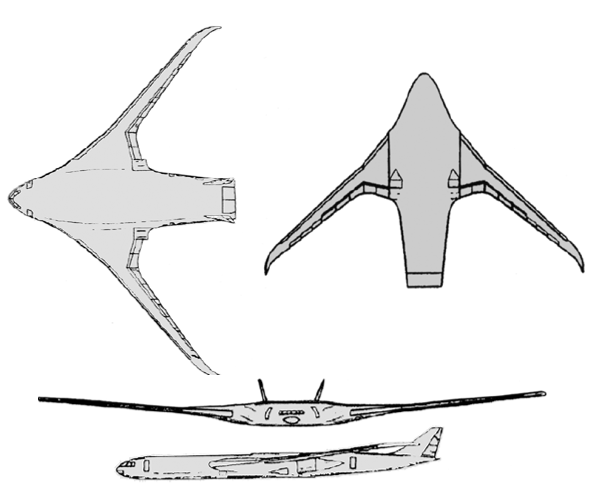
\includegraphics[scale=0.72]{Capitulo3/figs/2 6.png}
\caption{Following the first conceptualization of BWB, Liebeck and his McDonnell Douglas colleagues generated the transport configuration (first generation) in prototype. This served as the basis for later proposals such as BWB-450 after NASA X-48B \cite{Larrimer2020}}
\label{fig: primer concepto de Ala-Integrada}
\end{figure}
%
Bushnell mainly questioned the evolutionary step in the design of transport aircraft, highlighting that revolutionary development such as Boeing 707 and Douglas DC 8, the first generation of arrow-wing jets that revolutionized international air trade, had been successful by designs that follow a cautious, incremental and evolutionary pattern line. 
%
In the spring of 1989, nearly two dozen government and industry leaders, along with aeronautical academics and engineers and aerodynamics, gathered at NASA's LaRC to discuss possible new aircraft configurations. 
%
%\begin{itemize}
%    \item Preparar una aeronave como matriz de referencia\footnote{Sistema de coordenadas que se utiliza para definir la orientación y posición de montajes de componentes, distribución de cargas, ubicación de sistemas y otros aspectos de diseño, esenciales para la simulación y análisis de vuelo de aeronaves.} de acuerdo con la configuración TAW nombrada Transporte de Tecnología Sinérgica (\textit{Sinergistic Technology Transport ó STT n en inglés}) que sirva de base para unificar las filosofías de evolución y revolución en el diseño de aeronaves. 
%    \item A partir de la aeronave base \textit{STT}, proponer un diseño revolucionario con técnicas de optimización sin limitaciones
%    \item Comparar los resultados de aproximación de los dos diseños
%\end{itemize}
%
The Reference Matrix\footnote{Coordinate system used to define the orientation and position of component assemblies, load distribution, system location and other design aspects, essential for aircraft flight simulation and analysis.} according to the TAW configuration was named Transport of Synergistic Technology Transport or STT n in English with the aim of unifying the philosophies of evolution between the models of aircraft DC-10 and MD-11. Robert H.Liebeck together with his colleagues from McDonnell Douglas presented the aircraft of wing-integrated as a proposal of evolution and revolution, see Figure \ref{fig: primer concepto de Ala-Integrada}. The characteristics of the flight mission for the comparative analysis between STT and the first BWB concept were an operating range of 8,500 nautical miles with a capacity for 368 passengers travelling at a cruise speed of 0.85 Mach. The results showed a wide improvement in the first BWB concept over the STT, obtaining a ratio of 33.3 over 23.1, resulting in a fuel saving of 25.7 $\%$, \cite{Larrimer2020}.
%
Robert H.Liebeck concluded his study with the following note: \textit{the aircraft resulting from both concepts (revolution and revolution) offers such performance improvements on existing aircraft that we respond to NASA's question with a definitive YES}.
%
This was the beginning of the recognizable effort in designing, developing and testing prototypes in wind tunnel and flight testing of the BWB concept.


%En la Tabla \ref{tab: STT vs BWB} podemos observar la significativa optimización del concepto revolucionario de una aeronave de ala-integrada sobre la matriz de referencia \textit{STT} como concepto evolutivo. 
%
%\begin{table}[!h]
%\caption{STT comparado con BWB\cite{Larrimer2020}}
%\label{tab: STT vs BWB}
%\centering
%\begin{tabular}{ |p{4.5cm}||p{2cm}|p{2cm}|}
% \hline
% Características & STT & BWB \\
% \hline
% Diseño en millas nauticas & 8,500 & 8,500 \\
% Pasajeros & 368 & 368  \\
% Mach en crucero & 0.85 &  0.85 \\
% Motores & 3 VHBR & 2 VHBR \\
% Thrust (c/u) & 30,600 lb & 30,900 lb\\
% Envergadura & 188 ft & 260 ft \\
% Largo & 236 ft & 167  ft \\
% Área de ala & 2,020 $ft^2$ & 4,500 $ft^2$ \\
% Peso total & 367,200 lb & 338,800 lb\\
% Peso vacio operativo & 192,700 lb & 195,300 lb \\
% Levantamiento/Arrastre & 23.1 & 33.3\\
%Ahorro en combustible & base & 25.7 $\%$\\
% \hline
%\end{tabular}
%\end{table}
%


%%%%%%%%%%%%%%%%%%%%%%%%%%%%%%%%%%%%%%%%%%%%%%%%%%%%%%%%%%%%%%%%%%%
% Historia. líneas de tiempo y desarrollos BWB.

Following NASA's combined efforts, McDonnell Douglas and the leading pioneer in BWB configuration, Liebeck, revealed BWB's enormous potential to meet the airlines' ecological needs. 
%
Table \ref{tab: Desarrollos BWB en el mundo} shows the main BWB developments in the USA, Europe, Russia and China. Some of the BWB aircraft studied are shown in Figure \ref{fig: evolucion de BWB}.  
%
The latest BWB model from USA developed for flight testing was the \textbf{X-48C}. Its predecessors X-48 and X-48B were developed for wind tunnel testing and flight testing, respectively. 
%
On the USA side, from the origin of BWB they continued their research with BWB-tech projects. Later, McDonnell Douglas moved to Boeing and would evolve into the flight testing project for the model \textbf{X-48B}.
\begin{figure}[!h]
\centering
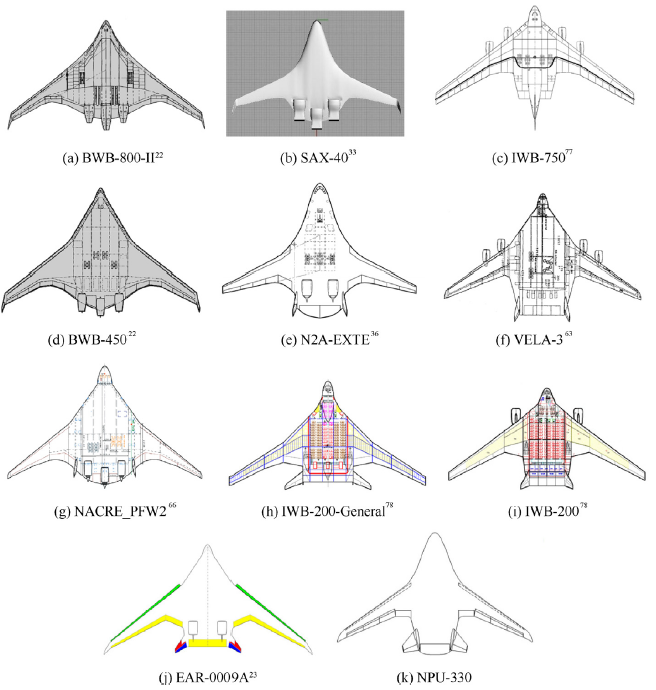
\includegraphics[scale=0.8]{Capitulo3/figs/2 7.png}
\caption{ Evolution of the concept of Wing-Integrated BWB \cite{CHEN2019}}
\label{fig: evolucion de BWB}
\end{figure}

\begin{table}[!t]
\caption{BWB Aircraft Development in USA, Europe, Russia and China \cite{CHEN2019}}
\label{tab: Desarrollos BWB en el mundo}
\centering
\begin{tabular}{ |p{1.9cm}|p{2.2cm}|p{2.5cm}|p{1.8cm}|p{1.9cm}|p{1.6cm}|  }
\hline
\multicolumn{6}{|c|}{BWB aircraft development} \\
\hline
Year & Proyecto & BWB-Nombre & Pasajeros & Rango(km) & Mach \\
\hline
\multicolumn{6}{|c|}{Main BWB projects in USA} \\
\hline
1994-1997 & BWB-tech & BWB-800-II & 800 & 13,000 & 0.85 \\
1997-2002 & Boeing & BWB-450 & 478 & 14,400 & 0.85 \\
2002-2012 & Flight test & X-48B & UAV & - & - \\
2003-2006 & SAI & SAX-40 & 215 & 9,300 & 0.8 \\
2007-2011 & SFW & N2A-EXTE & 262 & 11,100 & 0.8 \\
2010-2015 & ERA & ERA-0009A & 224 & 14,800 & 0.85   \\
2012-2013 & Flight test & X-48C & UAV & - & - \\
\hline
\multicolumn{6}{|c|}{Main BWB projects in Europe} \\
\hline
1998-2002 & Cranfield & BWB-98 & 960 & 14,200 & 0.85 \\
2000-2003 & MOB & BWB-MOB & - & - & 0.85 \\
2002-2005 & VELA & VELA-3 & 750 & 14,200 & 0.85 \\
2005-2010 & NACRE & NACRE & 750 & 14,200 & 0.85 \\
2008-2011 & ACFA2020 & ACFA-2020 & 470 & 13,300 & 0.85 \\
2015-2018 & AGILE & AGILE-BWB & 450 & 15,700 & 0.85 \\
2012-now & Airbus future & Airbus BWB & 470 & 13,300 & 0.85 \\
\hline
\multicolumn{6}{|c|}{Main BWB projects in Russia} \\
\hline
1997-2001 & 548-97 ISTC & IWB-750 & 750 & 13,700 & 0.85 \\
2014 &   & FW-200 & 211 & 16,000 & 0.85 \\
2019 &  & BWB-325 & 325 & 12,550 & 0.85 \\
\hline
\multicolumn{6}{|c|}{Main BWB projects in China} \\
\hline
2008-2017 & BWB & NPU-330 & 330 & 13,900 & 0.85 \\
\hline
\end{tabular}
\end{table}


%Los proyectos SAI, SFW y ERA proponían objetivos específicos en la investigación de BWB.
%Las siglas en inglés SAI refieren a la iniciativa para una \textbf{aeronave silenciosa}, dónde se implemento un sistema de propulsión de ingestión de la capa límite. 
%Las siglas en inglés SFW refieren a una aeronave subsónica de ala-fija. La intención con este proyecto era probar una aeronave híbrida BWB en túnel de viento que \textbf{minimizará la contaminación de ruido y emisiones}. 
%Las siglas en inglés ERA refieren a una \textbf{aviación ambientalmente responsable}, con el objetivo de minimizar el ruido, las emisiones y la quema de combustible para 2025.
%
%Poco después de que USA mostrará el potencial increíble de BWB, la Unión Europea comenzó sus propios desarrollos. El primer concepto que diseñaron era similar al propuesto por Boeing, y fue estudiado por la universidad de Cranfield. El diseño y desarrollo para aeronaves BWB fue progresivo y una sinergia entre distintos países de la Unión Europea, principalmente Francia y Alemania. 
%
%Por su parte, Rusia colaboró con USA y Europa para sus primeras conceptos de BWB, sustentados por el Centro Científico y Técnico Internacional (ISTC, en inglés) dónde lanzó IWB-750 de gran capacidad. %Las siguientes propuestas fueron para aeronaves más pequeñas. 
%
%Asimismo, China lanzó su investigación relativamente tarde, en 2008, dónde su primer versión fue para una capacidad de 150 pasajeros. Las siguiente versión fue para 300 pasajeros hasta llegar a su última versión propuesta para 330 pasajeros. 
%
%De acuerdo a lo anterior podemos concluir que desde el origen de BWB en USA, la investigación y desarrollo se ha llevado a cabo en sinergia entre USA y Europa principalmente. 


%%%%%%%%%%%%%%%%%%%%%%%%%%%%%%%%%%%%%%%%%%%%%%%%%%%%%%%%%%%%%%%%%%%%%%%%%%
% Prototipos para pruebas en túnel de viento y pruebas de vuelo

\section{Scale models - test benches}

Aircraft-scale model research plays a key role in the development of new real-scale configurations, being powerful tools for exploring the flight envelope. Some scale models for wind tunnel testing and flight testing are shown in Figure \ref{fig BWB prototipos}. 
%
\begin{figure}[h]
\centering
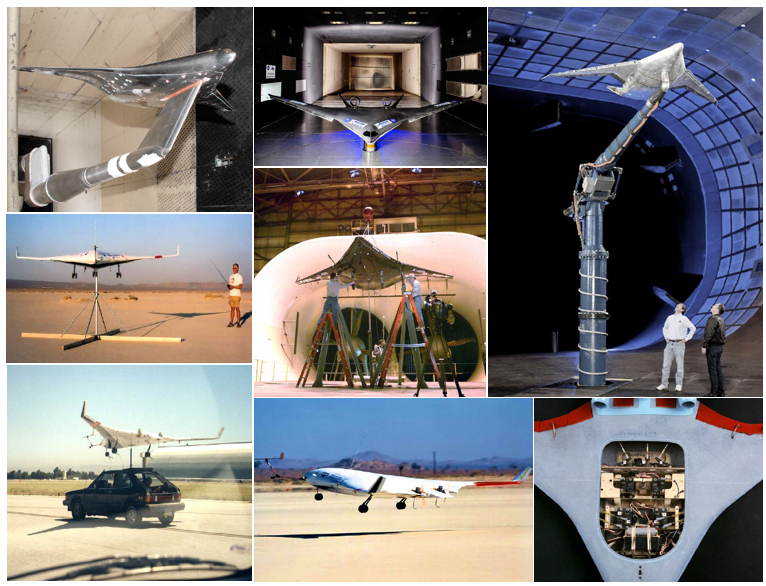
\includegraphics[scale=0.8]{Capitulo3/figs/2 8.png}
\caption{Wind tunnel scale models and flight and control tests \cite{Larrimer2020}}
\label{fig BWB prototipos}
\end{figure}
%
Now in 2023, the main aircraft manufacturing companies Boeing and Airbus after thirty years of research and development in the BWB aircraft model have a substantial advance in what appears to be the first BWB aircraft candidates for commercial flights such as X-48 B/C and MAVERIC, respectively. 

%%%%%%%%%%%%%%%%%%%%%%%%%%%%%%%%%%%%%%%%%%%%%%%%%%%%%%%%%%%%%%%%
% MAVERIC and X-48
%

\medskip


\textbf{Boeing X-48 B/C}\footnote{The challenge was to evaluate the flight mechanics of the BWB concept and prove that we can maintain stability and control. We comprehensively addressed these problems with X-48B and obtained excellent results. \textit{Robert H. Liebeck}.} 

%\textit{El reto era evaluar la mecánica de vuelo del concepto de Ala-integrada y probar que podemos mantener la estabilidad y el control. Abordamos exhaustivamente estos problemas con X-48B y obtuvimos excelentes resultados.} \textit{Robert H. Liebeck}. 
%
\begin{figure}[h]
\centering
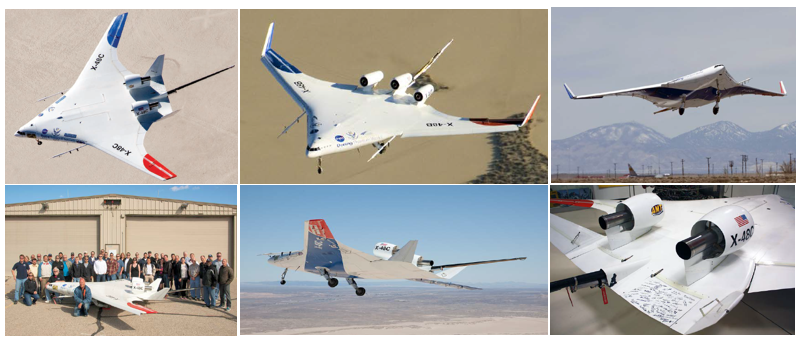
\includegraphics[scale=0.8]{Capitulo3/figs/2 10.png}
\caption{ Boeing X-48 B/C BWB \cite{Larrimer2020}}
\label{fig: Boeing X-48}
\end{figure}
%
%
The aircraft \textbf{BWB X-48B} is a prototype scale to 8.5\% The scale model has the same weight distribution as the actual model and allows simulations with the same moments of inertia and aerodynamic force coefficients, which allows validating stability and control as maneuver qualities. 
%Algunas características son:
%
%\begin{itemize}
%    \item Motores y sistema de combustible. Tres motores de gas turbofan JetCat USA P200 y una unidad de control de motores (ECUs). Cada motor produce 24.5kg de empuje a nivel del mar. Cada motor tiene su propio control de aceleración, de circuito de combustible y de bombeo de combustible. El tanque de gasolina de 47L permite una autonomía de 30-35min.   
%    \item Sistema eléctrico. 2 baterías de 32V y una de 6V. Una batería de 32V alimenta el subsistema de aviónica, incluyendo las computadoras de control de vuelo, el GPS y la unidad de medidas de inercia. La otra batería de 32V alimenta el sistema de actuadores excepto el timón que es alimentado por la batería de 6V. 
%    \item Sistema de navegación. Dos unidades de GPS. Uno mezclado con una unidad de medidas de inercia (IMU) para proveer altitud e información de navegación, y el independiente para proveer datos de posicionamiento. 
%    \item Aviónica y sensores. Se usaron sensores de alta calidad como un receptor de comando y un transmisor de enlace descendente de telemetría operados en el espectro de frecuencia de banda L. Una cámara en la nariz y un receptor de audio retransmitido en banda S. Un transponedor como identificador de posición para el tráfico aéreo. 20 sensores para las superficies de control conectados a la computador de control de vuelo. Dos booms de datos de aire miden la presión total, la presión estática, la temperatura estática y el ángulo de ataque como el ángulo de derrape. Un altímetro láser cambia las leyes de control de vuelo durante el despegue y aterrizaje, además de proveer lecturas de sobre el suelo con un altitud menor a 22m. Un IMU provee una alta precisión en tiempo real en posición y orientación con un sistema de navegación basado en datos GPS. Se añadió un segundo GPS. 
%\end{itemize}
%
%El modelo \textbf{X-48C} regresó a NASA DFRC en Octubre de 2009 después de un prototipo para túnel de viento en NASA Langley dónde se revisaron las modificaciones en estabilidad y control respecto a la versión X-48B. 
%
The main modifications in the X-48C version with respect to the X-48B version were: removing the fins with rudders at the tip and replacing them with a pair of vertical stabilizers on the adjacent platform where the engines are located. The three engines were replaced with a pair of 80kg AMT Titan turbofan gas engines, and the adjacent platform where the two engines and vertical stabilizers are located. 
%
Modifications were also made to the flight controller anticipating the maneuvering qualities and including flight controller restrictions to keep the aircraft in a safe flight envelope. 
%
To carry out the X-48B to X-48C Boeing improvements, it received USD 5.29 million from NASA for a one-year research programme aimed at identifying the concepts necessary for the BWB model to enter service in 2025, flying with lower noise and pollutant emissions and lower fuel consumption. 
%
The BWB X-48C concept was designated as a hybrid wing-fuselage aircraft (HWB) and its specific objective was to be the aircraft of the future to reduce fuel burning by 50\%, with 50\% less polluting emissions and 83\% Less noise. 
%

\medskip

\textbf{Airbus MAVERIC\footnote{BWB MAVERIC comes from the acronyms meaning: "Aircraft Model for Validation and Experimentation of Robust Innovative Drivers".}}\\
Airbus launched MAVERIC in 2017, starting its first flight tests in 2019 and continuing until the end of 2020. The scale version has a length of 2m with a wingspan of 3.2m. 
%BWB MAVERIC viene de las siglas en inglés que significan: "Modelo de Aeronave para la Validación y Experimentación de Controladores Innovadores Robustos". 
%
Although Airbus mentioned that they do not have a specific time for their BWB aircraft to go into service, they are firmly convinced that this new architecture for commercial flights will be the future for a sustainable aviation environment. Airbus’ MAVERIC BWB proposal is based on a hybrid propulsion of electric batteries and hydrogen cells in order to ensure zero emissions. 
\begin{figure}[h]
\centering
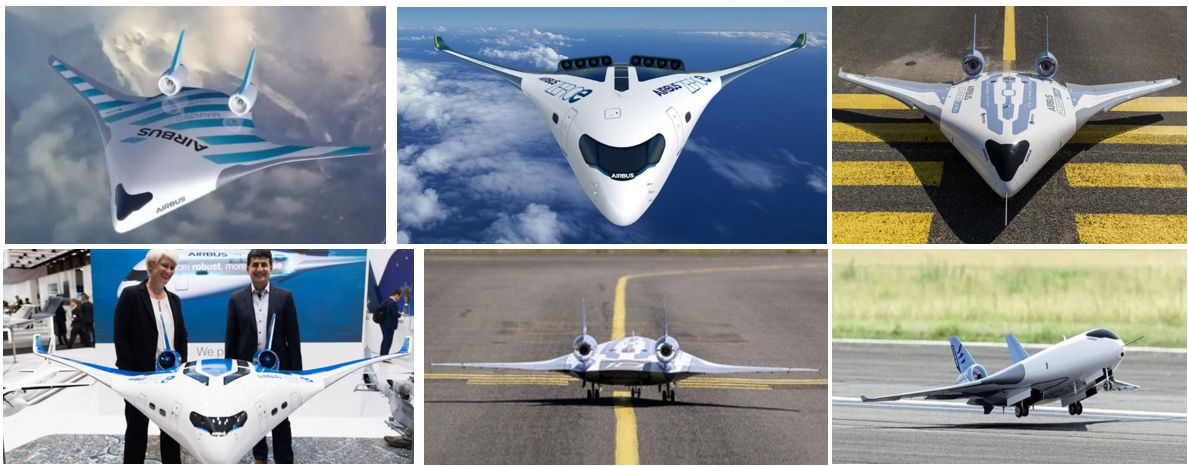
\includegraphics[scale=0.56]{Capitulo3/figs/2 11.png}
\caption{ Airbus MAVERIC BWB}
\label{fig: Airbus MAVERIC}
\end{figure}
%
%%%%%%%%%%%%%%%%%%%%%%%%%%%%%%%%%%%%%%%%%%%%%%%%%%%%%%%%%%%%%%%%%%%%%%%%%%
%%%% Ventajas/Desventajas BWB


%%%%%%%%%%%%%%%%%%%%%%%%%%%%%%%%%%%%%%%%%%%%%%%%%%%%%%%%%%%%%%%%%%%%%%%%%%%
\section{Flight Control Systems (FCS)}
%%%%%%%%%%%%%%%%%%%%%%%%%%%%%%%%%%%%%%%%%%%%%
%
A Flight Control Systems\footnote{,Flight Control System, FCS}, is a set of devices and programs that are used to control the trajectory, movement and stability of aerial vehicles. 
%
In general, the FCS is responsible for maintaining stability and control even under adverse wind conditions, turbulence, faults and other factors. 
%
The FCS for wing-integrated aircraft must include the following specifications:
\begin{itemize}
    \item  Digital Flight Control System with Total-Authority Fly-By-Wire (DFBW). The BWB configuration does not have the aerodynamic control surfaces in the horizontal and vertical stabilizers of an impenage, and therefore must rely on a digital flight control system with total-authority fly-by-wire (DFBW) for stability, control and flight routine in balance. The DFBW can work in synergy with a control allocation scheme to minimize actuators speeds, required forces of ACS and power requirements of all control inputs.
    \item Sensors. The FCS are equipped with a variety of sensors to measure the speed, altitude, direction, acceleration, temperature and other parameters of the aircraft. These sensors would also include gyroscopes and accelerometers to measure the orientation and inclination of the aircraft. 
    \item Actuators. The mechanisms that actuate the control effectors are called actuators. The BWB models have a greater number of control effectors, and therefore actuators. Actuators are connected to the aerodynamic control surfaces and the mechanisms of the vector thrust nozzle.
    \item Navigation System. It uses satellite signals to determine the position and trajectory of the aircraft, as well as a communication system that allows data transmission between the aircraft and air traffic controllers. 
    \item Software. The FCS includes advanced software that performs complex calculations and makes real-time decisions to maintain the stability and control of the air vehicle.
\end{itemize}
%
An initial analysis of the aerodynamic characteristics of BWB identified a potential failure in its sustained turns and post-exit modes with the nose upwards; both historical concerns with wing-flying and non-penetrating aircraft. This type of threat is of extreme importance. The potential behavior of a BWB aircraft has to be assessed at the edges of the low and high-speed levels of the envelope, including loss-input behavior, as well as possible falls, strokes and blows (a combination of these has destroyed Northrop YB-49A aircraft decades earlier).

\bigskip

%%%%%%%%%%%%%%%%%%%
\textbf{X-48 B/C}\\
NASA undertook flight investigations with the X-48B and X-48C aircraft at the NASA Dryden Flight Research Centre (DFRC) between 20 July 2007 and 9 April 2013. Both versions of vehicles completed a total of 122 remotely piloted flights (92 X-48B flights and 30 X-48 C flights). Each flight was in a range of 30-35 minutes. X-48B has 20 ACS coupled as control effectors for pitching, rolling and yawing moments, see Figure \ref{fig: Boeing X-48B ACS}. 
\begin{figure}[!h]
\centering
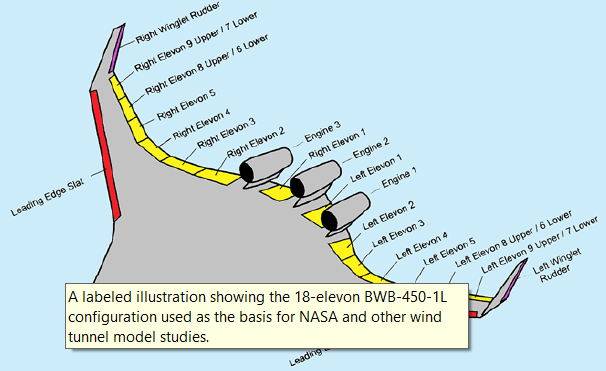
\includegraphics[scale=0.8]{Capitulo3/figs/2 23.png}
\caption{ Boeing X-48B with Aerodynamic Control Surfaces \cite{Larrimer2020}}
\label{fig: Boeing X-48B ACS}
\end{figure}
X-48B has a pair of lifts between its three engines, four pairs of elevons for the head and yaw combination, and two pairs of drag rudders that can act as aileron or speed brakes. Fins at the wing tip serve as vertical stabilizers and feature steering rudders.
%
%El programa de prueba de vuelo fue un esfuerzo hecho por NASA, la Fuerza Aérea de Estados Unidos, la compañia Boeing y Cranfield Aerospace. 
%
%La evaluación del programa de pruebas de vuelo para el X-48B buscó demostrar limitadores robustos del ángulo de ataque y deslizamiento lateral que proporcionarán resistencia de salida y permitieran maniobras agresivas hasta el $C_{Lmax}$ y un límite de deslizamiento lateral equivalente a un aterrizaje normal a gran escala en un viento cruzado de 35 nudos. 
%
In \cite{Larrimer2020} The tables of the six blocks of the X-48B and X-48C flight tests can be found, where the use of PID drivers is observed mainly, among others. 
%
For X-48 B/C three independent augmented systems (heading, rolling and yawing) work together the assignment control:
\begin{itemize}
    \item Enhanced longitudinal control and stability system (LSCAS)
    \item Increased control system and wire stability (RSCAS)
    \item Enhanced yaw control and stability system (DSCAS)
\end{itemize}
%
A deficiency in any control law would compromise the operations and stability of the entire system. For example, a higher demand for energy than is available would result in not having enough deflection of the ACS. 
%
%Las actividades que se esperan lograr mediante \textbf{asignación de control} en X-48 B/C son las siguientes: 
%\begin{itemize}
    %\item Comandar las ACS obteniendo los momentos desacoplados de cabeceo, roll y yaw demandados por el sistema de aumentado de estabilidad y control.
    %\item Generar las aceleraciones mínimas requeridas para las maniobras de estabilidad y control.
    %\item Proveer capacidades simultáneas en las aceleraciones del cabeceo y roll para las maniobras que requieren una ejecución simultánea, como recuperarse de regímenes de pérdida, que pueden envolver entradas simultáneas de cabeceo y roll para restaurar el control de vuelo de la aeronave BWB.
    %\item Minimizar la posición y la velocidad de los efectores durante el control aumentado.
    %\item Restringir las máximas posiciones y velocidades de las ACS para la asignación del control.
%\end{itemize}
%
The BWB configuration has to be as safe as the conventional TAW transport configuration, including demonstrating that it is a controllable vehicle in post-loss regions, an area where aircraft without impeneage or flying wings have experienced falls or flips. To counter subtract the mentioned Boeing design a control law concept based on the Versatile Control Augmented System (VCAS) architecture.
%
%El comando de seguimiento del vehículo aéreo X-48B en condiciones de post desplome con valores máximos en ángulo de ataque y ángulo de derrape funcionan bastante bien. El comando de seguimiento se predice con el análisis histórico usando una simulación de alta fidelidad de seis degrees de libertad, que también se utiliza para las pruebas de vuelo de los pilotos en tiempo real. Se llevo a cabo un análisis lineal del stick de cabeceo para el ángulo de ataque y de los pedales del timón de dirección para el ángulo de derrape, obteniendo las funciones de transferencia del modelo de lineal de tres degrees de libertad y también obteniendo buenos resultados con las Transformaciones de Fourier Rápidas (FFT) en las barridas de vuelo. 
%

 
In the X-48C version, the fins on the tips are replaced by central vertical stabilizers. This is because during the flight tests, the researchers faced unexpected control behaviors. In X-48B there were some oscillations and slip angles that were not expected. Directional stability was minimal due to the absence of vertical stabilizers, so they immediately did something about it. 

%La computadora de control de vuelo (FCC) procesa los comandos del piloto y los sensores de entrada para comandar las superficies de control. El sistema de control incluye un sistema de gestión de vehículo que integra guía y navegación, procesamiento de los sensores y los subsistemas del control de vuelo. La FCC registra aproximadamente 300 parámetros críticos a 200 hertz para la duración total de cada uno de los vuelos. 
%
%La estación de control de tierra (GCS) tenía cuatro operadores dentro de la unidad principal más tres estaciones de monitoreo externas. Los cuatro operadores eran el piloto, el oficial de seguridad de campo, el conductor de pruebas y el ingeniero de pruebas de vuelo. El piloto operó la aeronave usando controles convencionales de palanca, timón y acelerador. Las tres estaciones de monitoreo externas eran para el ingeniero de GCS, el operador de rastreo de vehículos y el ingeniero de margen de estabilidad en tiempo real. El GCS operaba en los siguientes tres modos: modo de vuelo de aeronave, modo de simulación de vuelo y modo de simulación de hardware. En el modo de vuelo, el piloto y la tripulación de vuelo controlaron la funcionalidad del X-48B de forma remota a través de los sistemas de telecomando y telemetría.
%El modo de simulación se utilizó para ensayar todas las misiones de vuelo antes de realizar las pruebas de vuelo reales. El modo de simulación de hardware se utilizó para verificar y validar nuevo software y para actividades de integración y validación de hardware.
%
%El modelo aerodinámico en la estación de control de tierra se basó en los datos reales del túnel de viento del vehículo y tenía una fidelidad superior. Esto permitió determinar ajustes de potencia específicos y ángulos de ataque y luego repetirlos con el X-48 real, mejorando así drásticamente la eficiencia de la prueba.
%
%La estación de margen de estabilidad en tiempo real (RTSM)  contenía una computadora de escritorio que ejecutaba el software MATLAB® (desarrollado por MathWorks, Natick, MA) que monitoreaba el sistema RTSM. Este sistema tenía la capacidad de procesar datos recopilados del flujo de telemetría casi en tiempo real. Esto permitió al operador de la estación ver los resultados inmediatamente después del procesamiento mientras la aeronave aún estaba en vuelo.
%
\bigskip

%%%%%%%%%%%%%%%%%%
\textbf{MAVERIC}\\
\begin{figure}[!h]
\centering
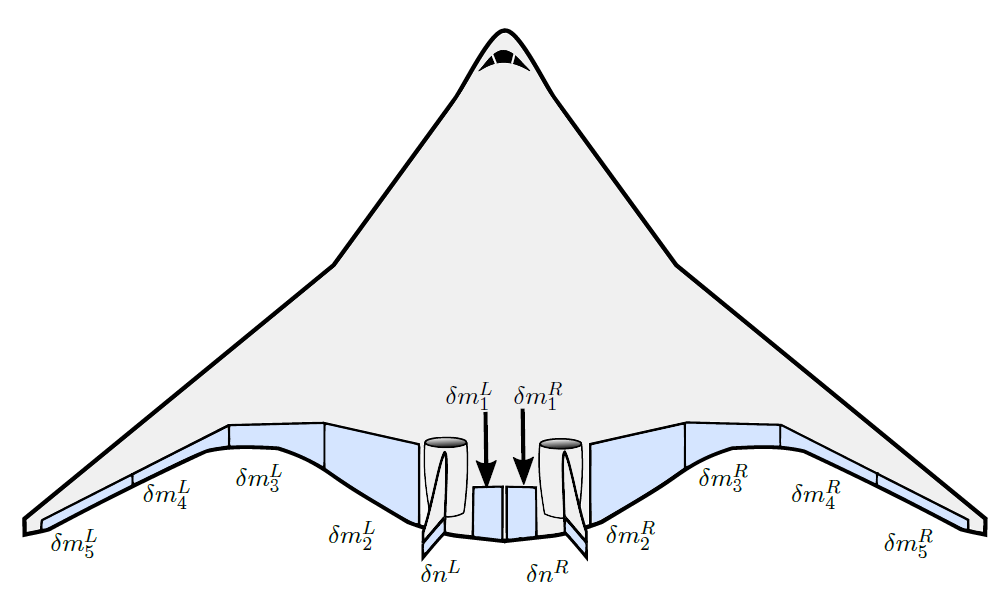
\includegraphics[scale=0.56]{Capitulo3/figs/2 12.png}
\caption{Airbus MAVERIC control surfaces \cite{Yann2016}}
\label{fig:  MAVERIC ACS}
\end{figure}
In \cite{Yann2016} the problem of the dimensioning of the control surfaces and the flight control system of an unstable BWB aircraft in closed loop are formulated and solved, using mathematical and numerical tools of the control community. In short, two alternatives were proposed for the iterative process:
\begin{enumerate}
    \item Integrated control design and actuator bandwidth.
    \item Integrated design of control and dimensioning of aerodynamic control surfaces. 
\end{enumerate}
%
The proposed methodologies were applied to the MAVERIC BWB longitudinal stability problem of Airbus using various assignment control techniques. \ref{fig:  MAVERIC ACS} the main ACS of MAVERIC are observed. It has ten ACS on the trailing edge (five per semi-wing) and a pair of steering rudders in its vertical stabilizers that are located above its engine pair.

\section{Discussion}

The aircraft concept of integrated wing represents a significant advance in aeronautical design by offering notable advantages in terms of aerodynamic efficiency and fuel economy.

The historical development of the BWB concept from its first experimental designs to the latest scale models proposed by Boeing and Airbus shows a trajectory of innovation and continuous improvement. Studying the evolution of the BWB provides a valuable perspective on the technical solutions adopted and the challenges overcome by engineers over time.

The construction and testing of scale models plays a crucial role in the validation and optimization of aircraft designs. Analyzing the methods and results of scale models provides essential information on aerodynamic and structural behaviour for future applications of larger dimensions.

The design of flight control systems specifically adapted to wing-integrated aircraft is essential to ensure stability and manoeuvrability. It highlights the assignment control technique for the control of wing-integrated aircraft. 

The detailed understanding of the background presented in this chapter provides the basis for the approach adopted in the design and control of the integrated wing aircraft proposed in this thesis. The knowledge gained from this background influences design decisions and the formulation of specific control strategies for this project.

Based on the background review, it is anticipated that the design and control of the wing-integrated aircraft will present stability and control challenges that will require robust controllers and ensure the stability of the closed loop. 


%
%La formalización del problema integra el diseño y control en la interacción de parámetros físicos, como las ganancias de las leyes de control,  el tamaño del stick y el ancho de banda de los actuadores. Lo más destacable es la integración del diseño y control como un problema de optimización acotado con criterios de dimensionamiento formulados como restricciones en la norma de frecuencia. 

%La segunda contribución es un diseño mejorado respecto a las metodologías tradicionales, dado que con menos iteraciones se logró un mejor diseño óptimo. Esta aplicación clarifica el campo de aplicación para aplicar la metodología en la etapa de diseño preliminar. 

%Se logró la formulación del problema de ancho de banda de los actuadores bajo la forma de $H_2 / H_\infty$ del problema de optimización, con restricciones en la trasferencia del lazo cerrado para asegurar adecuadas operaciones. 
%Esta formulación permitió encontrar el mínimo del ancho de banda que garantizará un cierto nivel de rendimiento. 

%Una segunda aproximación incluyó el momento de fuerza de la superficie de control en el criterio de optimización. Se encontró que una solución óptima para el consumo energético de los actuadores era estabilizar la aeronave utilizando las superficies de control más pequeñas, sin embargo, menos de 2.5 hertz son suficientes para controlar la inestabilidad. 
%Los elevons deben ser dimensionados no sólo con respecto a criterios longitudinales sino laterales. 
%
%Para sobrepasar esta limitación, propusieron un estudio de optimización conjuntando todas las superficies de control, incluyendo longitudinales y laterales leyes de control, tomando en cuenta los requerimientos estructurales de las leyes de control. 
%Para este propósito se requirieron modelos computacionales parametrizados para poder dimensionar. 
%
%Se hizo una representación en espacio de estados discreta de alta precisión con CFD.
%
%, para después aproximar en base a este modelo en una representación continua LFR usando aproximación por mínimos cuadrados. 
%
%La parametrización de espacio de estados no se hizo para parámetros de vuelo variantes o inciertos, más bien para el tamaño físico de las superficies de control, buscando obtener un modelo adecuado para futuras optimizaciones de controladores con ganancias. 
%
%La parametrización del espacio de estados obtenida se optimiza bajo restricciones de rendimiento de lazo cerrado y restricciones de calidad de maniobra.
%
% utiliza un enfoque de dominio de frecuencia para establecer estas restricciones de calidad de manejo, escritas como amplitud máxima y tasa de control en respuesta a entradas exógenas o perturbaciones. 
%Mientras este enfoque ya se ha desarrollado en la literatura, se propone una discusión sobre el significado y las limitaciones de estos criterios en el dominio temporal, que debería ser útil para el ingeniero dispuesto a aplicar nuestras técnicas para el dimensionamiento de aeronaves. Escribir el problema de la síntesis de ganancias bajo la forma de un problema de satisfacción de una sola restricción también es un paso importante y facilita las rutinas de optimización que tienen en cuenta las estructuras prescritas para los controladores. 
%Finalmente, una vez escritas correctamente estas restricciones, se proponen tres procedimientos alternativos de optimización para resolver el problema de cálculo de ganancias y parámetros físicos, diferenciándose cada uno de los demás por las variables proporcionadas al optimizador.
%Una primera síntesis considera una optimización desacoplada y secuencial de la ley de control de vuelo, y el tramo de superficies de control después, aprovechando que el módulo de asignación de control está parametrizado por el tramo de superficies de control.
%Si bien mostramos que este enfoque conduce a un diseño sub-óptimo, aún encontramos interés presentándolo desde una perspectiva de aplicación industrial: de hecho, este enfoque no requiere una optimización de ganancias a través de la síntesis H1: los ingenieros pueden aplicar cualquier técnica de síntesis a la que estén acostumbrados y optimizar los parámetros físicos con ganancias fijas en un segundo paso. 
 %El diseño inicial de las superficies de control ahora resulta viable, con un margen uniforme en el tamaño de las superficies de control con respecto a los criterios de calidad de maniobra especificados. 
 %Mostramos que el intervalo exterior de las superficies de control se puede reducir en un 45 \% antes de que se saturen las restricciones. Curiosamente, la mayoría de los puntos de vuelo en la envolvente de vuelo resultan estar dimensionados por un criterio de balanceo; sin embargo, en la mayoría de los puntos de dimensionamiento, a bajo número de Mach y gran altitud, también se dimensionan por rechazo de turbulencia, lo que implícitamente significa que el control de inestabilidad dimensiona la aeronave.
 %
%Finalmente se muestra una seria dependencia del diseño optimizado y el método de asignación de control: Incluir el método la asignación dentro de la optimización lleva a mejorar el diseño sólo en cierto porcentaje. 
%
%Como conclusión, esta técnica dimensiona una aeronave directamente desde las especificaciones de lazo cerrado, en la dinámica longitudinal y lateral. Esta técnica es capaz de entregar información relevante en el dimensionamiento sobre la envolvente de vuelo, y dimensiona los criterios de las cualidades de maniobra. 
%Esta metodología puede ser muy útil para los diseñadores al momento de hacer decisiones en la siguiente generación de aeronaves. 
%
%Desde el punto de vista teórico el uso de rutinas de optimización eficientes para sintonizar los controladores ha abierto de nuevo un tema bien conocido en la comunidad de control: ¿son los requerimientos para una ley de control confiables? y si no, ¿cuál es su máximo nivel de operación? en efecto, algoritmos de optimización han probado ser muy eficientes en encontrar la mejor solución para un conjunto dado de restricciones. El trabajo del diseñador de control evolucionó de sintonizar las leyes de control hasta las especificaciones de la sintonización. 
%Herramientas de decisión que le indiquen al diseñador si las restricciones son realizables es un campo de investigación atractivo. 
%
%La arquitectura acoplada de BWB sería una vez más un reto y una oportunidad para la exploración combinada de todos los casos posibles de falla: Es un reto porque un corte (por ejemplo, un actuador atascado) implicaría un degrado de operación en todos los ejes, haciendo el análisis muy complejo comparado con las prácticas actuales, y una oportunidad porque la redundancia de las superficies de control crearía una nueva arquitectura mucho más resiliente para el caso de fallas. 









